\documentclass[a4paper, 11pt, titlepage]{article}
\usepackage[utf8]{inputenc}
\usepackage[czech, english]{babel}

%\usepackage{natbib}
\usepackage{graphicx}
\usepackage{pdflscape}

\usepackage[unicode, colorlinks, hypertexnames=false, citecolor=red]{hyperref}
\addto\captionsenglish{\renewcommand{\figurename}{Obrázek}}
\addto\captionsenglish{\renewcommand{\tablename}{Tabulka}}

\begin{document}

\begin{titlepage}
    \centering 
    {\fontsize{25pt}{20pt}\bfseries
    VYSOKÉ UČENÍ TECHNICKÉ V~BRNĚ
    }
    
\includegraphics[scale=0.7]{./assets/fit-logo.pdf}
    \vspace{25pt}

    {\Large Modelování a simulace\\}
    \vspace{4pt}
    {\LARGE \bfseries 4) Uhlíková stopa v zemědělství, lesnictví a zpracovatelském průmyslu \\}
    \vspace{6pt}
    {\LARGE Využití lesa k~vyrovnání uhlíkových emisí a jeho udržení.}

    \vspace{180pt}
    {\Large 29.11.2019}\\
    \vspace{12pt}
    {\Large \bfseries Autor:\\}
    \vspace{12pt}

    \LARGE{
    \begin{tabular}{ l c r }
        Miroslav Válka & \texttt{xvalka05} \\
    \end{tabular}\\
    }
\end{titlepage}


\renewcommand{\contentsname}{Obsah}
\tableofcontents

\newpage
\section{Úvod} \label{sec:uvod}

V~této práci je řešena implementace lesa poutajícího uhlíkové emise z~atmosféry a jeho nezbytné udržování, která je použita pro~sestavení modelu\cite[snímek 7]{IMS_prez} lesa a stromové školky pro~obnovu lesa. 
Jedná se o~jednu z~problematik tzv. udržitelného lesního hospodářství.

Na základě modelu a simulačních experimentů\cite[snímek 10]{IMS_prez} bude možné pozorovat rozdíly sekvestrace uhlíku lesem pro~různé druhy stromů a zároveň schopnost stromové školky poskytovat sazenice pro omlazování lesa.

Smyslem experimentů je poukázat na~možnosti České~republiky pro~budoucí budování lesů, které by pomohly k~vyrovnávání uhlíkových emisí státu a díky tomu přispět jakožto členská země EU k~naplnění cíle ujednaného v Pařížské dohodě.\cite{EU_Paris_Agreement}

Pro~zpracování modelu bylo nutné nastudovat materiály o~uhlíkové stopě v~souvislosti se~stromy a lesy. Bohužel pro~pochopení daných materiálů bylo nezbytné začít základy, neboť autoři materiálů již počítají s~jistou znalostí v~oboru.

\subsection{Autor a zdroje informací}

Autor této práce je Miroslav Válka (xvalka05@stud.fit.vutbr.cz). K~vypracování práce byli využity zdroje a znalosti z~předmětu Modelování a simulace\cite[]{IMS_prez} na FIT VUT v~Brně. 

Pro~získání faktů a informací byly použity následující zdroje: "Carbon Footprint Measurement and Management: Case Study of the School Forest Enterprise"\cite{School_Forest_Enterprise}, "Growing trees to sequester carbon in the UK: answers to some common questions"\cite{Growing_Tree_in_UK}, "A life cycle greenhouse gas inventory of a tree production system"\cite{greenhouse}.

Při~zpracovávání práce byli také využity autorovi poznatky z~doby, kdy působil na~ZŠ~Újezd~u~Brna jako zástupce v~projektu Ekoškola~\footnote{https://ekoskola.cz/}. V~rámci této působnosti došlo k~návštěvě lesní školky spadající pod~Lesy města Brna~\footnote{https://www.lesymb.cz/lesni-skolky/}.


Pokusil jsem se kontaktovat zástupce, kteří pracovali na~publikaci "Carbon Footprint Measurement and Management: Case Study of the School Forest Enterprise"\cite{School_Forest_Enterprise} spadající pod~Českou zemědělsou univerzitu v~Praze, bohužel neúspěšně.
Dále jsem kontaktoval Lesy České republiky, s.p.\footnote{https://lesycr.cz/}, ale pouze se omluvili, že se mi nemohou momentálně věnovat a byl jsem odkázán na~jejich webové stránky, kde není nikde zmíněno, že by se české lesnictví v~současné době zajímalo o~uhlíkovou stopu. 

\subsection{Validace}

Validita\cite[snímek 37]{IMS_prez} byla ověřována během postupného testování a spouštění kalibračních experimentů. Výsledky kalibračních experimentů byly porovnávány s~již známými výsledky uvedenými v~publikacích, které byly zdrojem faktů.
Ověřování validity bylo považováno za~úspěšné ve~chvíli, kdy se výsledky simulace\cite[snímek 33]{IMS_prez} blížili hodnotám z~publikací (Hodnoty nemusí sedět přesně 1:1, protože výsledky v publikacích jsou zřetězeně zaokrouhlovány).
Více informací o~kalibračních experimentech naleznete v~kapitole Experimenty[Kapitola \ref{sec:simulacni_experimenty}].

\newpage
\section{Rozbor tématu} \label{sec:rozbor_tematu}

Jedena z~částí udržitelného lesního hospodářství je právě sekvestrace uhlíku ($C$) neboli pohlcování uhlíkových emisí z~atmosféry ($CO_2$) a uchovávání uhlíku ve~struktuře dřeva\cite{Carbon_in_Wood}. 
Různé druhy stromů pohlcují rozdílné množství uhlíku a mají rozdílnou životnost, proto je důležité správná volba stromů pro~založení lesa, který má efektivně snižovat koncentraci skleníkových [Tabulka \ref{tab:tree_uk}].\cite{Growing_Tree_in_UK}


\begin{table}[h]
    \centering
    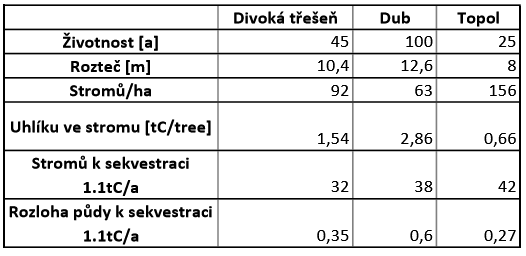
\includegraphics[scale=1]{assets/tab_stromy.PNG}
    \caption{Tabulka vybraných údajů o stromech z publikace\cite{Growing_Tree_in_UK}}
    \label{tab:tree_uk}
\end{table}

%\begin{table}[htb]
    %\centering
    %\begin{tabular}{|c|c|c|c|}
    %\hline
     %& Divoká třesen & Dub & Topol  \\ \hline 
    %\hline
    %Životnost ($a$) & 45 & 100 & 25 \\ \hline
    %Rozteč ($m$) & 10.4 & 12.6 & 8 \\ \hline
    %Stromů/ha & 92 & 63 & 156 \\ \hline
    %Uhlík v celém stromu ($tC/tree$) & 1.54 & 2.86 & 0.66 \\ \hline
    %Počet stromu k sekvestraci $1.1tC/a$ \footnotemark & 32 & 38 & 42 \\ %\hline
    %Rozloha půdy k sekvestraci $1.1tC/a$ & 0.35 & 0.60 & 0.27 \\ \hline
    %\end{tabular}
    %\caption{Tabulka údajů o stromech z publikace\cite{Growing_Tree_in_UK} (Jen nezbytné)} %\label{tab:sometab}
%    \label{tab:tree_uk}
%\end{table} 
%\footnotetext{Jednotka $ 1.1tC/a $ se čte jako \textit{tun uhlíku za rok}.}

Stromy během svého života projdou několika etapami při~kterých se různí v~lesnictví jejich přínos/podíl na~uhlíkových emisích. Pro~vypěstování sazenice ze semínka v stromové školce jsou generovány uhlíkové emise \cite{School_Forest_Enterprise}. Ty jsou taktéž generovány při vysazování sazenic do~lesa \cite{School_Forest_Enterprise}. Až během růstu a stárnutí stromu dochází k~zaznamenatelné sekvestraci uhlíku. 

Překročení životnosti stromu neznamená okamžitou smrt stromu, ale pouze uvádí od~kterého roku života se objevuje šance na~jeho úmrtí. Tato šance není přesně daná, ale zdroj uvádí roční úmrtnost v~rozsahu $3.5\%-5.1\%$ \cite{Tree_Lifespan}. 

Uchovávání uhlíku ve~struktuře dřeva si klade za~cíl vypěstovat strom a ten následně nechat zpracovat a nahradit jiným dříve než~zemře. Použitelnost mrtvých stromů je převážně jako palivo a v~tom případě dojde k~vrácení uzamčeného uhlíku zpět do~atmosféry. Nejlepším řešením využití stromů je přepracování do~výrobků nebo staveb s~dlouhou životností.\cite{Carbon_in_Wood}

Výsadba stromů do~lesa neprobíhá celoročně, ale jen v~určitých měsících a to převážně na~jaře.\cite{School_Forest_Enterprise}

Pro~stromové školky údaje nejsou jednotné a velmi se od~sebe liší a to i v~rámci různých let. Produkované uhlíkové emise pro~stromovou školku v~Česku s~rozlohou $6900ha$, produkcí sazenic $2000000$ kusů je $99kgCO_2/ha$\cite{School_Forest_Enterprise}. 
Produkované uhlíkové emise pro~stromovou školku ve~Švédsku je v~rozsahu $47-133kgCO_2$ na~$1000$ sazenic, ale v~USA se jedná o~rozsah $29-40kgCO_2$ na~$1000$ sazenic\cite{greenhouse}.


\subsection{Popis použitých postupů}

Pro~implementaci simulačního modelu\cite[snímek 44]{IMS_prez} byl vybrán jazyk C++ a to konkrétně ve~standardu C++11 a simulační knihovna SIMLIB\cite{simlib}. Hlavním důvodem výběru je široká podpora platforem na~kterých je možné simulaci zprovoznit. Dále knihovna SIMLIB je pod~licencí GNU~LGPL a je možné ji využívat zdarma bez~poplatků. Knihovna SIMLIB poskytuje kompletní simulační prostředí\cite[snímek 38]{IMS_prez} pro~diskrétní\cite[snímek 32]{IMS_prez} simulaci.


\subsection{Popis použitých metod/technologií}

Pro~kompilaci zdrojových kódu C++ je používán kompilátor g++. K řízení sestavení programu je používán GNU Make. 
Knihovna SIMLIB byla získána z~oficiálních webových\cite{simlib}. Autory této knihovny jsou Petr Peringer, David Leska a David Martinek.

\newpage
\section{Koncepce} \label{sec:koncepce}

\subsection{Návrh konceptuálního modelu\cite[snímek 48]{IMS_prez}}

Do~našeho modelu\cite[snímek 7]{IMS_prez} zavedeme jisté abstrakce a odprostíme se od~přílišně detailní reality. 

V~prvé řadě zjednodušíme náš pohled na~stromy, neboť nás nezajímají přesné hodnoty stromů, ale zajímají nás souhrnné hodnoty celého lesa. Každý strom pro~nás bude průměrným stromem, nebudeme brát v~potaz, že reálné stromy mají různě velké plochy pro~příjímání uhlíkových emisí a ani individuální podmínky ve~kterých strom žije. Životní etapy v lese rozdělíme na tři etapy růst stromu, žití stromu a dožívání stromu, kde součet etapy růstu a žití dává dohromady životnost stromu [Kapitola \ref{sec:prilohy} Přílohy: Obrázek~\ref{fig:pn_forest}, \sloppy Čas~růstu=Time(R), \sloppy Čas~žití=Time(Z)].

Zároveň všechna získaná fakta vždy operují s~časovou jednotkou roky, ale ta je pro~nás příliš veliká a mohla by zanášet do~simulace znatelné chyby zapříčiněné synchronizací procesů [Kapitola \ref{sec:prilohy} Přílohy: Obrázek~\ref{fig:pn_forest}, \sloppy Čas~měření=Time(M)]. Z~tohoto důvodu zvolíme za~časovou jednotku měsíce a upravíme hodnoty faktů pro~námi zvolenou časovou jednotku. Zároveň provedeme přepočty z~uhlíku na~uhlíkové emise [Tabulka \ref{tab:propocet}].


\begin{table}[h]
    \centering
    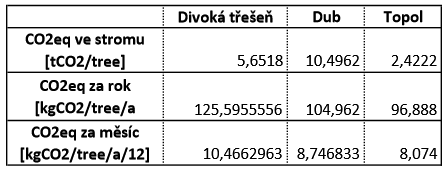
\includegraphics[scale=1]{assets/tab_prepocet.PNG}
    \caption{Tabulka přepočítaných hodnot pro stromy}
    \label{tab:propocet}
\end{table}

V~našem modelu se nebudeme zabývat kácením stromů a jejich zpracováním, které produkuje uhlíkové emise, ale pouze jejich pěstováním. Ale i přesto budeme monitorovat počty mrtvých stromů, neboť u~nich s~jistotou víme, že v~nich vázaný uhlík se kompletně vrátí zpět do~atmosféry.

Informace o~uhlíkové stopě stromové školy v Česku přepočteme na~1000 sazenic.
Po~přepočtu to dělá $341.55kgCO_2$ na 1000 sazenic za rok.
V~porovnání jsou mezi státy příliš výrazné rozdíly. Jelikož model má ukázat možnosti pro~Česko, tak budeme brát v~potaz údaje české stromové školky, které si ale ještě převedeme na~hodnotu pro~jednu sazenici za~měsíc. Na~jednu sazenici nám padá $0.0284625kgCO_2$ za~měsíc. 


\subsection{Formy konceptuálního modelu}

Pro~znázornění konceptuálního modelu\cite[snímek 48]{IMS_prez} byla vytvořena Petriho síť\cite[snímek 61]{IMS_prez}, která je rozdělena na~dvě části. První část Petriho sítě [Kapitola \ref{sec:prilohy} Přílohy: Obrázek~\ref{fig:pn_forest}] zobrazuje životní cyklus stromů rostoucích a žijících v~lese. Druhá část Petriho sítě [Kapitola \ref{sec:prilohy} Přílohy: Obrázek~\ref{fig:pn_nursery}] představuje základní stromovou školku, která pěstuje a dodává sazenice stromů.

Pro~výpočty kapacity stromů v~lese i kapacity sazenic ve~stromové školce je použit přepočet využívající dostupnou rozlohu pro~pěstování v~hektarech a rozteče mezi stromy/sazenicemi v~metrech.
$$trees[pcs]=\frac{area[ha]*10^4}{spacing[m]^2}$$

Vztah pro~převod uhlíku uloženého ve~stromu na~ekvivalentní množství oxidu uhličitého.\cite{Growing_Tree_in_UK}
$$1C=3.67CO_2$$

\newpage

\section{Architektura simulačního modelu/simulátoru} \label{sec:architektura_simulacniho_modelu_simulatoru}

\subsection{Mapování abstraktního modelu do simulačního\cite[snímek 36]{IMS_prez}}

Simulace začíná vybráním a nastavením scénáře, který nastavuje vstupní podmínky pro~simulační experimenty a také počáteční stav.
Scénáře experimentů zprostředkovává jmenný prostor \textit{scenario}.
Následuje vytvoření a naplánování trojice generátorů \textit{PlantingSeedlingsGenerator, PlantingTreesGenerator, NeedTrees}. 
Generátor \textit{PlantingSeedlingsGenerator} vytváří a spouští jednou za~čas rutinu pro~výsadbu nových sazenic ve~školce. 
Generátor \textit{PlantingTreesGenerator} vytváří a spouští jednou za~čas rutinu pro~výsadbu nových stromů v~lese z~dostupných sazenic ve~školce.
Poslední \textit{NeedTrees} slouží k~vytváření a spouštění požadavků o~stromy.
Po~dokončení simulace jsou vytisknuty výstupy a to buď zkráceně (Výstupy důležité pro~zvolené experimenty) a nebo podrobné (Jsou vytisknuty veškeré nasbírané informace během simulace).

Implementace stromové školky byla vytvořena podle abstraktního modelu Petriho sítě stromové školky [Kapitola \ref{sec:prilohy} Přílohy: Obrázek~\ref{fig:pn_forest}].
Třída \textit{Seedling} představuje proces sazenice ve~stromové školce. Vyrostlé sazenice, které jsou dostupné pro~výsadbu, jsou uchovávány ve~frontě \textit{GrownSeedling}, kde čekají dokud nedojde k~výsadbě do~lesa nebo nedojde k~jejich přestárdnutí. Jednou za~čas dochází k~událostem \textit{PlantingSeedlings}, které představují cykly výsadby nových sazenic. Nově vysazené množství je vždy závislé na~množství aktuálně pěstovaných a spravovaných sazenic ve~školce a to tak, aby nedošlo k~překročení kapacity školky.

Implementace lesa byla vytvořena podle abstraktního modelu Petriho sítě lesa [Kapitola \ref{sec:prilohy} Přílohy: Obrázek~\ref{fig:pn_forest}].
Třída \textit{Tree} představuje proces stromu v~lese. Strom prochází až třemi etapami života. Tyto etapy jsou mladý les, vzrostlý les a starý les. Stromy dávají vědět okolí v~jaké etapě života se nachází svojí přítomností ve~frontách k~tomu určeným \textit{YoungForest, GrownForest, OldForest}. 
Stromy opouští les pokud umřou nebo pokud jsou vydány na~požadavek o~storm. 

Požadavky na~stromy jsou obstarávány třídou \textit{NeedTrees a NeedTree}. Při příchodu požadavku na~strom/stromy jsou z~lesa odebírány stromy a to v~pořadí od~nejstaršího. Přednostně tedy odchází stromy ze~starého lesa u~niž existuje šance na~úmrtí a následně ze vzrostlého lesa. Pokud les nemá k~dispozici dostatečně starý strom pro~splnění požadavku, tak odchází požadavek jako neuspokojený.
Během života starých stromů ve~starém lese může dojít k~jejich úmrtí a uvolňují tak místo pro nové stromy.

Výsadba nových stromů probíhá jednou za~čas při události výsadby \textit{PlantingTrees}. Vysazujeme stromky dokud platí následující pravidla. Vysazujeme stromy v~případě, že je dostupná jeho sazenice a zároveň v~lese je volné místo pro~jeho výsadbu. V~opačném případě přerušujeme výsadbu.  

%Minimálně je nutno ukázat mapování abstraktního (koncept.) modelu do simulačního (resp. simulátoru). Např. které třídy odpovídají kterým procesům/veličinám a podobně.


\newpage
\section{Simulační experimenty} \label{sec:simulacni_experimenty}

Účelem kalibračních experimentů je ověřit správnost chování simulačního modelu v~rámci známých údajů z~publikacích.

Cílem experimentů je ukázat možnosti sekvestrace uhlíkových emisí lesem pro~různé druhy stromů a poukázat nejen na různou efektivitu pohlcování uhlíkových emisí, ale~i na~vedlejší efekty způsobené výběrem druhu stromu a omlazováním lesa. Mezi vedlejší efekty řadíme:
\begin{itemize}
    \item Nadbytečná/Nedostačující produkce sazenic.
    %\item Poměr (ne)dostupného zdravého dřeva pro trh.
    \item (Ne)úspěšné uzamykání uhlíku do dřevěných produktů.
\end{itemize}

\subsection{Postup}

\subsubsection{Postup pro kalibrační experimenty}

Kalibrační experimenty ověřují chování simulačního modelu po~částech a jejich identifikátory mají prefix \textit{K} následovaný číslem. 
Fakta z~niž model vychází pochází z~různých nezávislých zdrojů a proto tyto experimenty se provádí nad~vstupy a výstupy brané v~kontextu ke~konkrétním zdrojům faktů.
\begin{itemize}
    \item \textit{K1, K2, K3, K4, K5, K6}
    \begin{itemize}
        \item Cílem je ověřit správnou sekvestraci uhlíku lesem v~časovém horizontu života stromů.
        \item Ve~výchozím stavu budeme mít plný les složený ze~zvoleného druhu stromu.
        \item Vstupní hodnoty pro~experimenty [Tabulka \ref{tab:kalibracni_exterimenty_vstupy}] vychází z~tabulky \ref{tab:propocet}.
    \end{itemize}
    \item \textit{K7, K8, K9}
    \begin{itemize}
        \item Cílem je ověřit zda strom obsahuje stejné množství uhlíku jako uvádí zdroje u~stejně starých stromů.
        \item Ve~výchozím stavu budeme mít plný les složený ze~zvoleného druhu stromu.
        \item Vstupní hodnoty pro~experimenty [Tabulka \ref{tab:kalibracni_exterimenty_vstupy}] vychází z~tabulky \ref{tab:propocet}.
    \end{itemize}
\end{itemize}

\begin{table}[htb!]
    \centering
    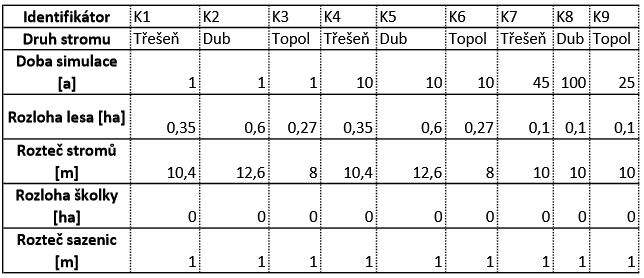
\includegraphics[scale=0.8]{assets/tab_ke_K1_K9_in.PNG}
    \caption{Tabulka hlavních vstupních hodnot pro kalibrační experimenty}
    \label{tab:kalibracni_exterimenty_vstupy}
\end{table}

\newpage
\subsubsection{Postup pro experimenty}

V~experimentech si ukážeme chování pro~různé druhy stromů při~změně maximálního počtu odebíraných stromů za~rok v~časovém horizontu $300let$. Odebíráním stromů uvolňujeme místo pro~mladé stromky a omlazujeme les. Budeme pozorovat výsledné $CO_2$, které je pro~nás rozdílem mezi odebranými uhlíkovými emisemi lesem bez~uhlíku uloženého v~mrtvých stromech a uhlíkových emisí vyprodukovaných lesní školkou. Opakujeme experimenty dokud výsledné $CO_2$ nezačne klesat nebo pokud se začne opakovat s~přesností na~jednotky $tCO_2$. Ve~výchozím stavu je les z~poloviny naplněn mladými stromy. Pro~náše experimenty důležité vstupní hodnoty naleznete v~tabulkách [Tabulka \ref{tab:experimenty_vstupy_1}] [Tabulka \ref{tab:experimenty_vstupy_2}].

\begin{table}[htb!]
    \centering
    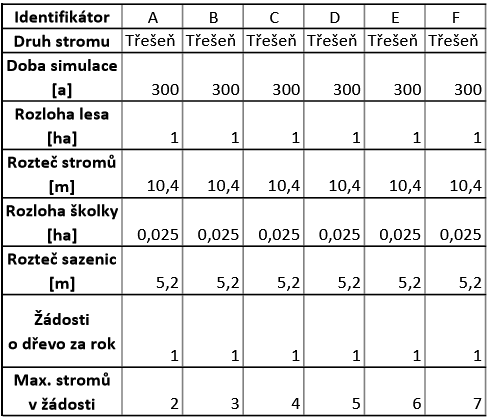
\includegraphics[scale=1]{assets/tab_e_A_F_in.PNG}
    \caption{Tabulka vstupních hodnot pro experimenty A-F}
    \label{tab:experimenty_vstupy_1}
\end{table}

\begin{table}[htb!]
    \centering
    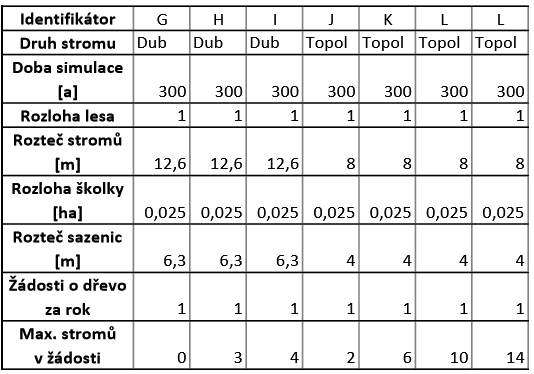
\includegraphics[scale=1]{assets/tab_e_G_M_in.PNG}
    \caption{Tabulka vstupních hodnot pro experimenty G-M}
    \label{tab:experimenty_vstupy_2}
\end{table}

\newpage

\subsection{Dokumentace simulačních experimentů}

\subsubsection{Kalibrační experimenty}

\begin{table}[htb!]
    \centering
    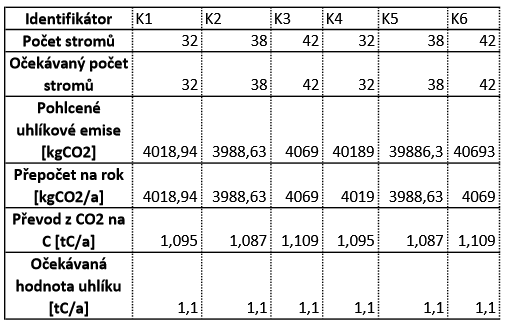
\includegraphics[scale=1]{assets/tab_ke_K1_K6_out.PNG}
    \caption{Tabulka výstupních hodnot pro kalibrační experimenty K1-K6}
    \label{tab:kalibracni_experimenty_vystupy_1}
\end{table}


\begin{table}[htb!]
    \centering
    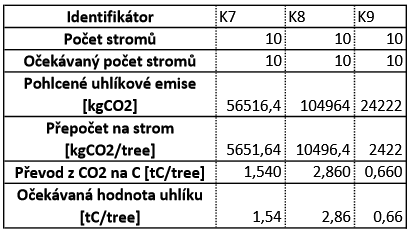
\includegraphics[scale=1]{assets/tab_ke_K7_K9_out.PNG}
    \caption{Tabulka výstupních hodnot pro kalibrační experimenty K7-K8}
    \label{tab:kalibracni_experimenty_vystupy_2}
\end{table}

\newpage
\subsubsection{Experimenty}

\begin{table}[htb!]
    \centering
    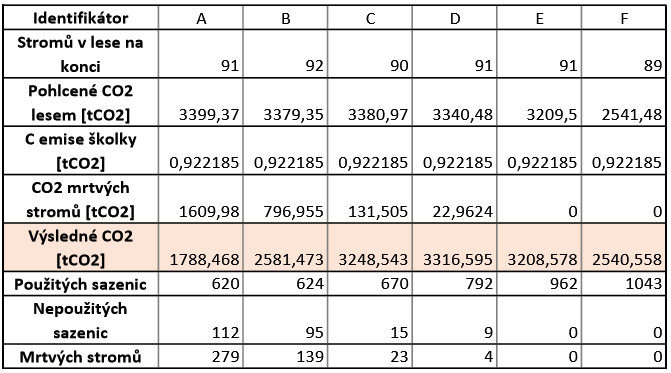
\includegraphics[scale=0.8]{assets/tab_e_A_F_out.PNG}
    \caption{Tabulka výstupních hodnot pro experimenty A-F}
    \label{tab:experimenty_vystupy_1}
\end{table}

\begin{table}[htb!]
    \centering
    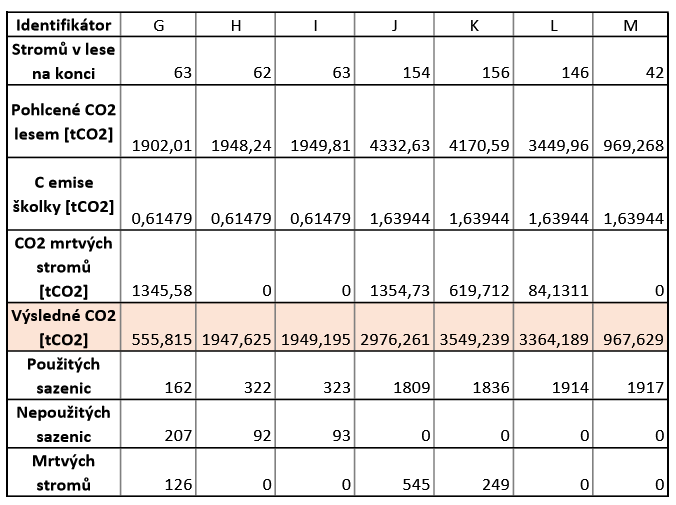
\includegraphics[scale=0.8]{assets/tab_e_G_M_out.PNG}
    \caption{Tabulka výstupních hodnot pro experimenty G-M}
    \label{tab:experimenty_vystupy_2}
\end{table}

\newpage
\subsection{Závěr experimentů}

Úspěšně bylo provedeno 22 experimentů z~toho 9 kalibračních. Během kalibračních experimentů jsme ověřili věrohodnost modelu, kdy se nám výsledné hodnoty u~první sady kalibračích experimentů liší jen o~zaokrouhlení [Tabulka \ref{tab:kalibracni_experimenty_vystupy_1}] a u~druhé sady kalibračních experimentů došlo ke shodě [Tabulka \ref{tab:kalibracni_experimenty_vystupy_2}]. Z~toho vyplývá, že jedna ze~stran (já nebo autoři publikace) počítali se~zaokrouhlovací chybou.

Během dalších experimentů jsme mohli pozorovat výsledné snížení uhlíkových emisí z~atmosféry [Tabulky \ref{tab:experimenty_vystupy_1} a \ref{tab:experimenty_vystupy_2}], kde na~tento jev má dominantní vliv nejen výběr druhu stromu, ale i~vhodné omlazování lesa daného druhu stromu. 

V~tomto směru nám pokračování v~podobném experimentování nepřinese další pro~nás zajímavé výsledky, neboť experimenty zachycují stavy s~nadmírou mrtvých stromů [Tabulka \ref{tab:experimenty_vystupy_1}, sloupec A; Tabulka \ref{tab:experimenty_vystupy_2}, sloupce G a J], ideální stav s~minimem mrtvých stromů [Tabulka \ref{tab:experimenty_vstupy_1}, sloupce D a E; Tabulka \ref{tab:experimenty_vystupy_2}, sloupce H, K a L ] a~i~stav přílišné poptávky po~dřevu s~následkem snižování stromů v~lese [Tabulka \ref{tab:experimenty_vystupy_1}, sloupec F; Tabulka \ref{tab:experimenty_vystupy_2}, sloupec M].   

\newpage
\section{Shrnutí simulačních experimentů a závěr} \label{sec:shrnuti_simulacnich_experimentu_a_zaver}

Z~výsledků experimentů vyplývá, že ze~zvolených stromů lépe vychází druhy stromů, které sice mají kratší životnost, ale jejich výhodou je jejich menší košatost, kdy se jich na~stejně velkou plochu vleze více. Ale oproti druhům stromů s~dlouhou životností je nutné je ve~vetším počtu nahrazovat novými stromy a je tedy s~nimi více práce a práce není zadarmo. 

Validita modelu byla ověřena při~kalibračních experimentech, kdy se výsledné hodnoty lišili oproti referenčním jen o~zaokrouhlení na~řád desetin $tCO_2$. 
V~rámci projektu vznikl simulační model lesa poutajícího uhlíkové emise z~atmosféry a stromové školky pro~obnovu lesa, který vychází ze~získaných informací uvedených v~kapitole Rozbor tématu a byl implementován v~programovacím jazyce C++. 


% Z výsledků experimentů vyplývá, že ... při předpokladu, že ... Validita modelu byla ověřena ... V rámci projektu vznikl nástroj ..., který vychází z ... a byl implementován v ...
 
\newpage
\bibliographystyle{czechiso}
\renewcommand{\refname}{Literatura a zdroje}
\bibliography{references}

\newpage
\section{Přílohy} \label{sec:prilohy}

\begin{figure}[ht!]
    \centering
    %\includegraphics[scale=0.8,angle=-90,origin=c]{assets/les-Les_v3.pdf}
    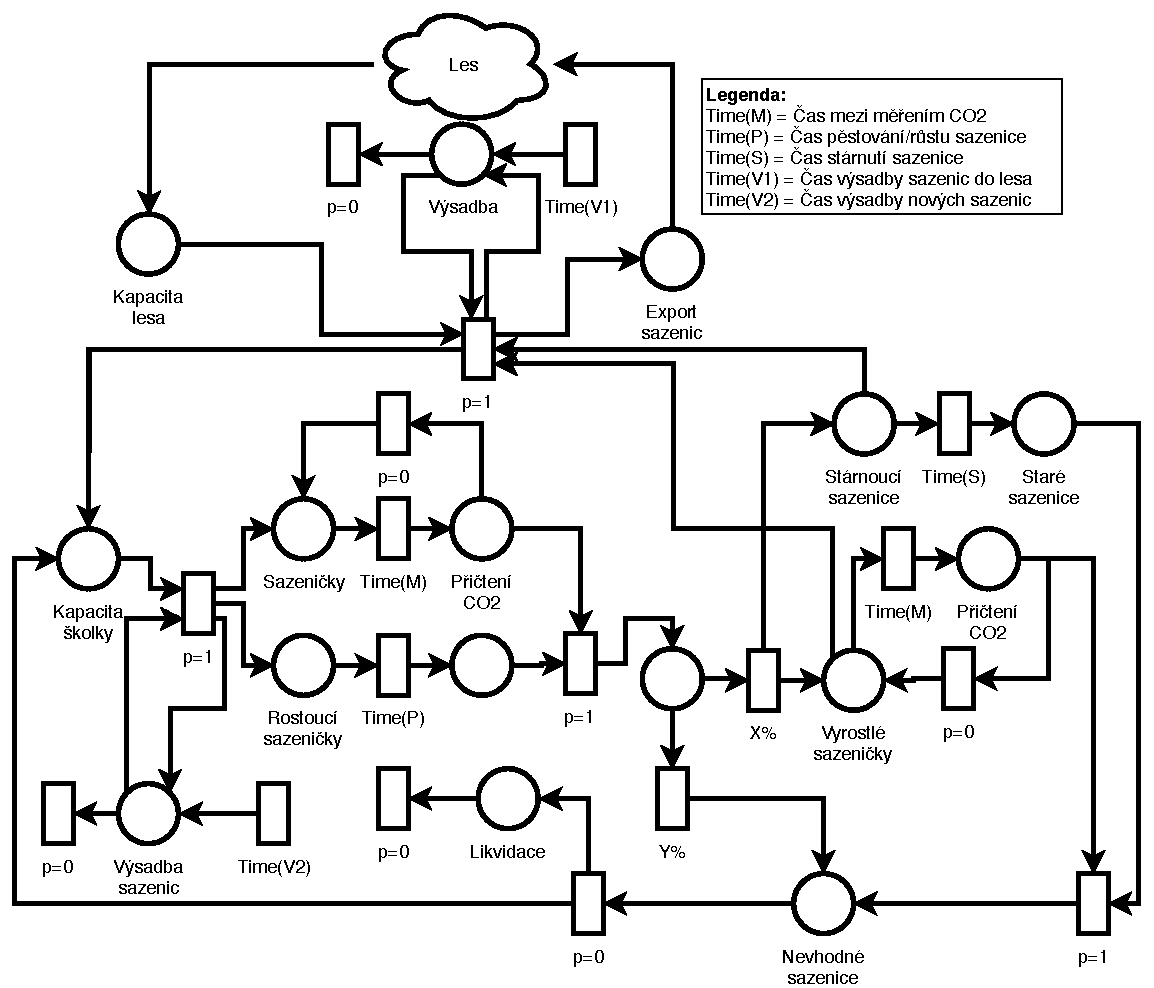
\includegraphics[scale=0.65]{assets/pn_skolka_v2.pdf}
    \caption{Petriho síť modelu lesa (2. část: Stromová školka)}
    \label{fig:pn_nursery}
\end{figure}

\begin{landscape}
\begin{figure}[!ht]
    \centering
    %\includegraphics[scale=0.8,angle=-90,origin=c]{assets/les-Les_v3.pdf}
    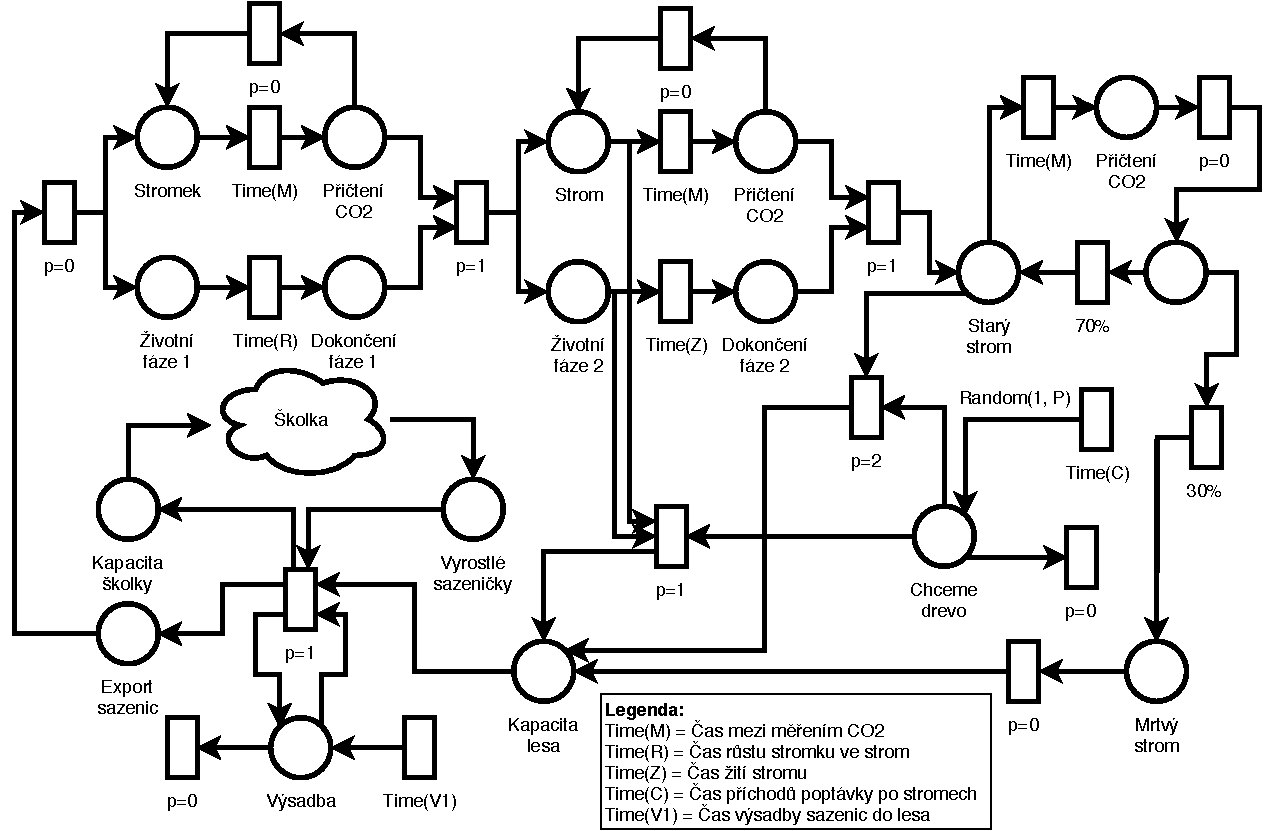
\includegraphics[scale=0.85]{assets/pn_les_v2.pdf}
    \caption{Petriho síť modelu lesa (1. část: Les)}
    \label{fig:pn_forest}
\end{figure}
\end{landscape}


\end{document}
